\documentclass[../../main.tex]{subfiles}

% Uses images 218, 220

\begin{document}

\newchapter{Project Review}{project-review}

\section{Design and manufacture} \label{sec:project-review:design-and-manufacture}

Since components of the avionics subsystem had been procured throughout the design phase, an iron bird could be constructed to ensure that all the necessary components were properly wired and compatible.
The iron bird model is shown in Figure \ref{fig:iron-bird}, modelled on the wiring diagram \ref(Figure {fig:wiring-diagram}), and built onto a miniaturised cutout of the same general shape as the full-size aircraft.
While not all of the servos were included in the iron bird, each servo group was represented.
The iron bird also gave a much clearer indication of roughly how much wiring would be needed to connect the various groups.

\importimage{iron-bird}{iron bird.}{Iron bird}{0.7}

Limited manufacturing of the final model occurred before physical work on the project was halted.

Most notably, models of the PUC were sent for printing.
Initially only one was sent, with the intention of its being a prototype to negate the risk of spending budget on designs that had errors.
This first print was successful and resulted in a full additively manufactured PUC \ref{fig:puc-printed}.

\importimage{puc-printed}{PUC, printed in SLS nylon.}{SLS nylon PUC}{0.5}  % TODO: reposition

The signal splitters could also be manufactured, seen in Figure \ref{fig:manufactured-splitters}.
This was a fairly quick process of cutting down the copper stripboards and soldering header pins to them in the correct locations, and was done alongside the soldering of the signal output pins and jumper wires to the flight controller.

\importimage{manufactured-splitters}{each of the manufactured splitters.}{Manufactured splitters}{0.8}

Although the full electronics system was never assembled in the UAV due to the COVID-19 pandemic, almost all of the necessary physical components were purchased and manufactured, and their compatibility was tested in the iron bird. 

\section{Testing and Evaluation} \label{sec:project-review:testing-and-evaluation}

As it can be seen in Figure \ref{fig:layout-variations}, there is a significant difference in weight between configurations.
Ballast was employed to maintain a constant weight, the placement range, maximum and required ballast configurations can be seen in figures \ref{fig:ballast-details} to \ref{fig:max-ballast}.
In doing so, the results gathered from the flight tests would not be biased by the weight differences.
Furthermore, the position of the ballast along the fuselage was dictated by the centre of gravity position for each layout.
The shift in CG without the influence of ballast can also be seen in Figure \ref{fig:layout-variations}.
The wingtip pusher and nose-mounted motor was set to be the weight and CG position datum.
This decision was taken since this one is the heaviest configuration, presenting the most rearwards centre of gravity. 
\importimage{ballast-details}{Mass and CG details with maximum and required ballast to achieve a stable configuration, and range of positioning along UAV mounting tray}{Ballast details}{0.9}
\importimage{required-ballast}{Plot of ballast placement range along normalised mounting tray length. Note: Value in range is ballast mass, value in green is CG location in terms of MAC prior to ballast addition, value in blue is the mass of the aircraft with the ballast.}{Required ballast}{0.9}
\importimage{max-ballast}{Plot of ballast placement range along normalised mounting tray length. Note: Value in range is ballast mass, value in green is CG location in terms of MAC prior to ballast addition, value in blue is the mass of the aircraft with the ballast.}{Maximum ballast}{0.9}
\importimage{layout-variations}{CG and mass change for each layout, not accounting for ballast; standard configuration is marked in red.}{Variation between configurations}{0.9}
\importimage{flight-test-plan}{flight test plan, listing all configurations which would be tested.}{Flight test plan}{0.9}

\subsection{Flight test} \label{sec:project-review:testing-and-evaluation:flight-test}

\importimage{puc-locations}{enumeration of all possible power unit positions on the UAV.}{PUC positions}{0.9}

Figure \ref{fig:puc-locations} shows all possible configurations of PUCs, with each side of the table as each side of the wing, except for D and E which are the fuselage locations.
Blue areas show where both wings have the same configuration and so data can be recorded for that overall layout during a flight with that configuration; green is the initial configurations that would be tested in a knockout format in order to minimise the number of flights required to find the best configuration with the D and E calls as green/blue because they are in both; red is repeats of the lower half of the matrix; and black is for impossible configurations due to both being fuselage locations.
It should be noted that D and E cannot be doubled up either, so where D is on both wings, that is a configuration of only one motor on the nose and the same for E.
There are however configurations where a fuselage motor is combined with a wing motor: this would create an unbalanced aircraft due to an off centre CofG so in these cases the wing motor would be applied to both wings and the UAV would be flown with three motors, the fuselage motor acting as a safety backup in the case of a wing motor failing.

\importimage{knockout-table}{knockout table for determining the best configuration with minimal runs.}{Knockout table}{0.8}

The knockout table (Figure \ref{fig:knockout-table}) shows the matchups of wing power unit locations required to find the best PUC configuration, but no data for each location would be recorded due to the mixing of configurations, and so an additional flight of the best configuration would be required in order to compare it to the fuselage motor locations, totalling twelve flights.
Also, any flights where the distance along the span of the wing is different for the two power units would be difficult to give definitive results due to the off centre CofG.
This would induce a rolling moment and so a constant application of ailerons would be needed to counteract this, which would itself induce a small yawing moment.
This would affect the results because the way of finding the better configuration would be to measure the yaw angle in flight, with the more efficient location being on the opposite side to the direction of yaw, and so any influence on the yaw angle coming from the CG would not help. 

If the power unit locations were all flown symmetrically, however, the aircraft data could be recorded for each one in order to compare post flight, and the differences in power usage at a constant flight velocity would show which location was the most efficient.
Only twelve total flights would be needed, as shown in Figure \ref{:figpuc-locations}, which is the same number of flights as the knockout method, just with a more accurate method of comparison.
This is therefore the method chosen for the testing of the UAV.

The process for testing would involve flying one configuration to accumulate the required data, then changing the batteries while changing the configuration and downloading flight data from the microcontroller.
The next configuration would then be flown, and the used batteries put on charge.
The order of flights is shown in Figure \ref{fig:flight-order}. 

\importimage{flight-order}{list of the planned flights, in order, with the configurations and batteries used.}{Flight order}{0.7}

There would be three sets of batteries for the wing motors, and two sets for the fuselage motors, so that multiple flights could be flown while the used batteries are recharging, reducing delays.
The first three flights would be different wing motor configurations, then one of the fuselage motor configurations would be flown to give the wing batteries extra time to charge before three further flights of the wing configurations.
The wing tip configurations would need to be flown with the nose motor in order to have control in a wing tip motor failure situation, and so these would require three batteries to be used, limiting the charge time of the batteries used in the final flight.

\subsection{CFD} \label{sec:project-review:testing-and-evaluation:cfd}

Alongside the wind tunnel test, CFD simulations were used to assess the validity of the airframe of the UAV.
Furthermore, the wind tunnel results provided data to validate the results of the simulations.
The software used for the simulation was Star-CCM by Siemens.
Using a polyhedral mesh with refinement blocks placed in the key areas such as the wing tip and the flaps (Figure \ref{fig:cfd-mesh}) the residuals exhibited from the simulations were on the order of $10^{-7}$.
The turbulence model used for those simulations was the K-epsilon model.
The flow was assumed to be steady and incompressible.
The difference in the results between the wind tunnel tests and the CFD simulations floated around \pc{8} for both drag and lift loads.
This difference can be attributed to the presence of the struts in the wind tunnel test as well as inaccuracies present in the wind tunnel model.
The minor increase in the difference was exacerbated as the angle of attack of the UAV increased; the maximum was up to \pc{10} difference.
As the angle of attack increases the adverse pressure gradient on the suction surface of the wing increases as the boundary layer thickness does.
Hence the flow is closer to stall conditions; the case in which the turbulence model's inherent errors might more obviously feed into the results.
This explains the increase in the difference between the results shown in Figure \ref{fig:empirical-numerical-comparison}. 

\importimage{cfd-mesh}{section view of the polyhedral mesh utilised for CFD simulations.}{CFD mesh}{0.7}

Through the validation of these results the quality of the flow over the final model of the UAV could be analysed (Figure \ref{fig:flow-behaviour}).
A non-powered version was analysed in flight conditions exhibiting an overall lift of \newtons{77}.
Furthermore, the takeoff conditions were simulated to ensure that the high lift devices were performing as designed.
At takeoff speed of \mps{13}, flaps deployed at \degr{20} incidence and \degr{5} angle of attack, the UAV achieves the required $C_\mathrm{L,max}$ for takeoff. 

\importimage{empirical-numerical-comparison}{comparison of physical wind tunnel results with numerical CFD results.}{Comparison of methods}{0.9}

Simulating the interaction between the airframe and the flow arriving from the propeller required more computational power due to the use of a rotating reference frame.
This tool allows the recreation of the rotation of the propeller by imposing a rotating flow domain within the free moving flow domain.
A separate cylindrical domain is created around the propeller, the diameter of this is set as twice the one of the propeller.
Furthermore it extends both forward and backwards of the propeller by \pc{25} of its diameter.
This method was first verified against the results gathered from the propeller wind tunnel test.
A difference of \pc{10} was observed from the real results for the case of \mps{15} wind speed and 11500 RPM, with residuals on the order of $10^{-5}$.
This difference can be attributed, in part, to the inaccuracies present in the CAD model of the propeller due to the lack of accurate data describing its geometry.
Furthermore, a second source of errors are, as aforementioned, the inherent approximations of the turbulence model used.
The decision to carry out simulations with CAD models was made due to the lack of reliable sources providing accurate models or data of the propeller's geometry.
A simulation recreating the conditions described in \cite{kroo-86}, where the propeller swirl interacts with a wing section, shows an increase in propeller efficiency equal to \pc{8}, which is consistent with the results found in the paper.

% \importimage{propellor-flow}{propellor flow structure.}{Propellor flow}{0.3}
% \importimage{trailing-edge-flow}{flow quality at the trailing edge during takeoff.}{Trailing edge flow}{0.3}
% \importimage{flap-flow}{flow behaviour with flaps deployed at 20 degrees incidence.}{Flap flow behaviour}{0.3}

\begin{figure}[H]

    \centering
    \begin{subfigure}[b]{0.49\columnwidth}
        \centering
        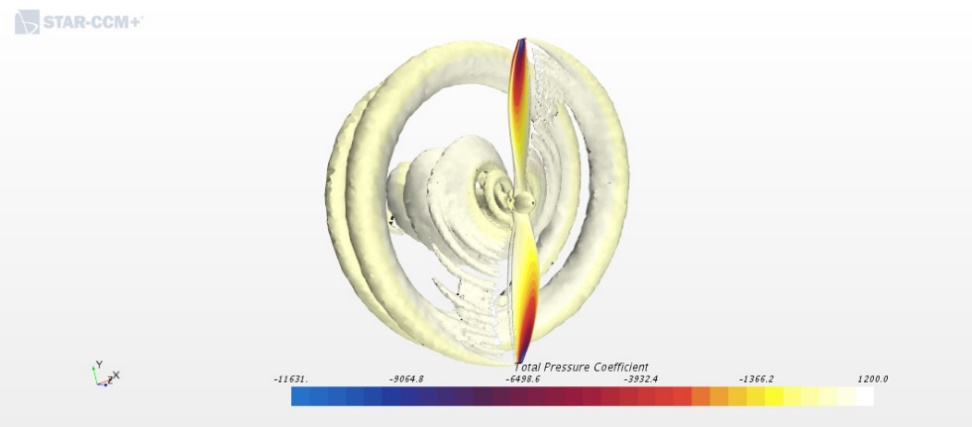
\includegraphics[width=\textwidth]{propellor-flow}
        \caption{Propellor}
        \label{fig:flow-behaviour:propellor}
    \end{subfigure}
    \hfill
    \begin{subfigure}[b]{0.49\columnwidth}
        \centering
        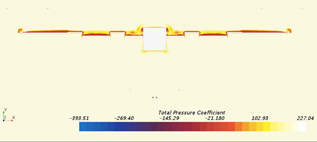
\includegraphics[width=\textwidth]{trailing-edge-flow}
        \caption{Trailing edge}
        \label{fig:flow-behaviour:trailing-edge}
    \end{subfigure}

    \begin{subfigure}[b]{0.49\columnwidth}
        \centering
        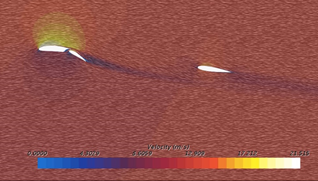
\includegraphics[width=\textwidth]{flap-flow}
        \caption{Flaps}
        \label{fig:flow-behaviour:flaps}
    \end{subfigure}
    
    \caption{results CFD simulations showing flow behaviour at various locations of interest; (c) has flaps deployed at 30 degrees.}
    \label{fig:flow-behaviour}
\end{figure} 

\section{Budget} \label{sec:project-review:budget}

As parts were designed and the construction of the model was established, different elements were added to the budget in order to keep track of costs.
This included both costs for parts that would later be needed and estimations of costs for parts whose exact prices were unclear early in the design process.

One difficulty found was the cost of 3D printed parts, as the estimations made for the costs of these parts was significantly lower than the final cost.
This was due primarily to the change from PLA to ABS and Nylon construction, and also the requirement to use a certain supplier for 3D printing funded by the grant, which was much more expensive than other suppliers originally explored.
This meant that at the time of printing (just as the university shutdown happened) the cost of the 3D printed parts increased significantly, and the material of a few of the additively manufactured parts needed to be changed to keep costs down.
This meant that either the strength of these parts was reduced, or the design was modified to accommodate for the change in material, resulting in an increase in weight.
With a larger budget, more nylon could be used to print the aircraft, thereby keeping its weight down. 

\importimage{budget}{complete budget table.}{Budget table}{0.9}

The final budget is shown in Figure \ref{fig:budget} and it shows costs that were realised in black text, and items that were budgeted for but were never bought due to the university shutdown in blue text.
The budget was maximised as much as possible in order to cover the costs of the 3D printing, but the 3D printing budget itself was not fully accounted for, with over £85 remaining, due to the limitations on suppliers of nylon-printed parts, which increased that part's cost by around \pc{100} for Nylon SLS parts; and more for ABS or PLA parts.
This meant that other parts could not be made using this budget as they would go overbudget, and there was no option of supplementing the costs from another part of the funding.

The university funding was fully allocated, with much of the spending being on parts and supplies for the wind tunnel model, with the carbon fibre parts ordered just before the university shutdown while it was still thought that the building of the final flight model would be possible.
The external funding is also fully accounted for, with the parts ordered being the initial purchases for the electronics of the flight model, along with the expendable flight vehicle that was to be used for testing of the avionics and autopilot. 

\section{Impact of Covid-19} \label{sec:project-review:impact-of-covid-19}

\subsection{Progress to March} \label{sec:project-review:impact-of-covid-19:progress-to-march}

By 13th March, the final design was essentially finished and parts were in the process of being ordered, or finalised for procurement (such as 3D printed or foam cut parts).
The presence and slow initial onset of the outbreak in the UK altered the schedule somewhat, and these would have likely been finished earlier without it.
Initially the group went ahead in the hope that restrictions may be lifted in time to resume construction and testing, so one of the many 3D printed parts was ordered as a test piece; but it soon became clear that lockdown would remain for an extended period of time and the model would be unable to be built for testing.
At this point the focus shifted onto finalising the design, both in CAD and mathematically, and the supporting administrative work (ensuring budget would still be met despite not being used), so that this could be effectively communicated in the project outputs. 

The thin green lines (Figure \ref{fig:gantt-chart}) show what had actually been completed relative to initial timeframe estimates.
As can be seen for some activities, the project was behind schedule.
This can be partly attributed to planning and unforeseen circumstances such as the wind tunnel being fully booked much further ahead in time than had been anticipated, resulting in the schedule being set back due to testing not being possible until after Easter.
Once confidence in the design had increased to the point of willingness to fly without a wind tunnel test, the window for physical testing widened considerably. 

\subsection{Adjustments around restrictions} \label{sec:project-review:impact-of-covid-19:adjustments-around-restrictions}

Once restrictions were put in place, the group quickly shifted to meetings over Skype, and then Microsoft Teams, both as a group and with supervisors.
These were held mostly held weekly once everyone had settled back into routine, so that communication between the project team and project supervisors could be maintained.
With regards to the project, the focus quickly shifted from what had been an attempt to build and test towards to maximising efficiency as a group to work on the project outputs; and work quickly began on polishing CAD models and mathematical work (represented by the lines extended beyond the outbreak announcement, Figure \ref{fig:gantt-chart}) to be presented in the report, presentation, and video.

\subsection{Planned future work} \label{sec:project-review:planned-future-work}

By the time of the university's closure, it was already clear that the final model would not be build, and the group had moved away from the original schedule.
Had the COVID-19 outbreak not happened, however, the project would have looked very different from what it looked like on March the 13th, and what it looks like now.
As seen in Figure \ref{fig:gantt-chart}, there are two feasible plans in a non-COVID-19 scenario: either based on the original project plan, or what had happened to date.
The thin green lines show what had been completed, and it can be seen that some activities were behind schedule (any missing before the purple line are unknown or unimportant to this section).
Had the order to stop not come through, mathematical and CAD aspects of the design would have been finalised by approximately the end of the thin green line for 'final model design', which is where the project finished initially.
Work past that shown in 'mathematical analysis' and 'CAD design' are mostly a result of polishing, though a minor change to the tailplane mounting angle (by \degr{0.2}, not significant enough to be a problem) did occur as a result.  

The thin red lines show the team's estimate for what would have occurred had the outbreak not happened based on what had been completed already, and the purple line shows the date of the early end of term.
Procurement had already begun, and many of the 3D printed parts, foam cut parts, electronics, avionics, and fasteners has been finalised.
Many had been ordered or were prepared to be ordered before it became clear that a manufactured model was infeasible.
Other parts that were being finalised up to the design finish date would have been ordered as soon as they were ready.  

\importimage{gantt-chart}{initial plan compared with how the project progressed and what would have happened next.}{Gantt chart}{0.9}

The original plan was to have construction and testing complete by Easter and to be making project deliverables over Easter, to submit by the original deadline.
Instead, however,the construction of the UAV would have been finished over Easter, and work would have begun on aspects of the report, video, and presentation where possible, prior to inserting aspects about the final construction and testing into all three.
The team respects that this is off the original plan, and that it would have been more of a crunch time, however it is felt by all $-$ including the project supervisor $-$ that it would have been possible, and up to the end the team were proceeding as though it would have been: planning new days for wind tunnel testing after Easter, flight test days with the RC plane group, and internal tests with a pilot who would be paid for his services.  

At the start of the project the team was made aware of the potential for commercial progression.
Ideally, had the wind tunnel or flight tests been completed and results shown that changes were required, these would have been documented and worked upon through analytical processes, CFD, FEA, and iteration in CAD to produce a refined concept of the next UAV.
At the conclusion of design, the budget was projected to be near its limit; the team therefore would not have been able to produce a second model based on further design work.
Had the results and further design work shown enough promise, however, the team could have worked further with Dr. Kirk to continue the production at a commercial level, with the intention of eventually expanding the scale of the design; or another team could have picked up where this design left off and continued the process of design, testing, and refinement on another GDP budget. 

\section{Conclusion} \label{sec:project-review:conclusion}

This project intended to identify the most efficient power unit location on the body of a conventional airframe through the flight testing of a UAV with a movable propulsion unit.
Despite the steady design progress made by all team members, the manufacture and flight testing of the UAV was not possible due to the COVID-19 lockdown.
The project was on course to achieve its objectives, however, and to complete the desired outcomes.  

The final design has been shown to meet the requirements set out in the project brief.
The model incorporates reconfigurable propulsion units on the wings and fuselage to allow the testing of multiple propulsion unit locations.
This allows for an informed decision on the most efficient configuration.
An early design was tested both physically in the wind tunnel and mathematically.
The final design was tested in CFD, FEA, and mathematically to confirm its airworthiness, allowing for the confidence that the proposed design would be a strong and stable flight platform for the necessary tests.
The construction of the UAV was planned to be simple to allow for fast changes of the power unit configuration as specified by the hardware requirements. 

Thorough testing of the electrical systems showed that the UAV would be fully controllable by a pilot, whilst recording the necessary data during the flights to determine the most efficient propulsion unit location.
Unfortunately, the autopilot functionality could not be tested due to the lockdown.  

The vision for this project does not end with its conclusion, however.
Dr. Kirk's ambition was to obtain a model UAV that would function as a test bed to provide research for future electrical aircraft development, and there is significant further work that can be built upon the foundations laid out by this project.
With the completion of the manufacture and testing of the design laid out in this report, followed by the refinement of a maximum efficiency design based on the results of those tests, the sky is the limit for the ELMO UAV. 

\end{document}
